\section{The map, and does it matter?}
\label{sec:map}

\begin{figure*}[t]
\centering
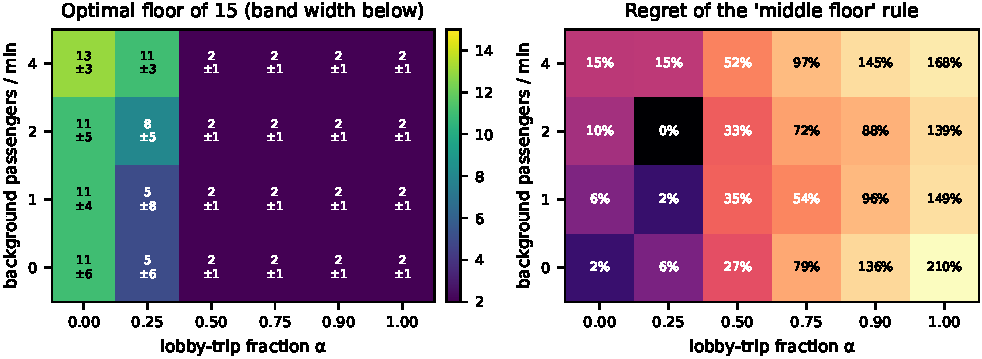
\includegraphics[width=\textwidth]{figures/map.pdf}
\caption{\RobN-floor building, one car parked at the lobby, stairs on. Left:
optimal floor over lobby-trip fraction and background rate, with the width of
the 5\% indifference band beneath each value. Right: regret of the
middle-floor rule in the same cells.}
\label{fig:map}
\end{figure*}

Figure~\ref{fig:map} puts the pieces on one grid. In \RobCellsFloorTwo\ of
\RobCells\ cells --- every cell with $\alpha \ge 0.5$ --- the optimum is the
lowest residential floor, and its indifference band is a single floor. The
middle floor is competitive only along the left edge: at $\alpha = 0$ the
optimum is the median (\RobHZeroZero\ at zero traffic, band
\RobBandZeroZero) drifting up to \RobHZeroFour\ under saturation; at $\alpha =
0.25$ it is floor \RobHQuarterZero\ at zero traffic and rises with load to
\RobHQuarterFour, with a band that spans \RobBandQuarterFour\ at 4/min --- the
one regime where the honest answer is ``it does not matter''. Everywhere to
the right the middle-floor rule costs tens to hundreds of percent
(\RobRegMidHalfZero\% at $\alpha = 0.5$, \RobRegMidNineOne\% at $\alpha =
0.9$ with 1/min, where the top floor costs \RobRegTopNineOne\%).

\begin{figure*}[t]
\centering
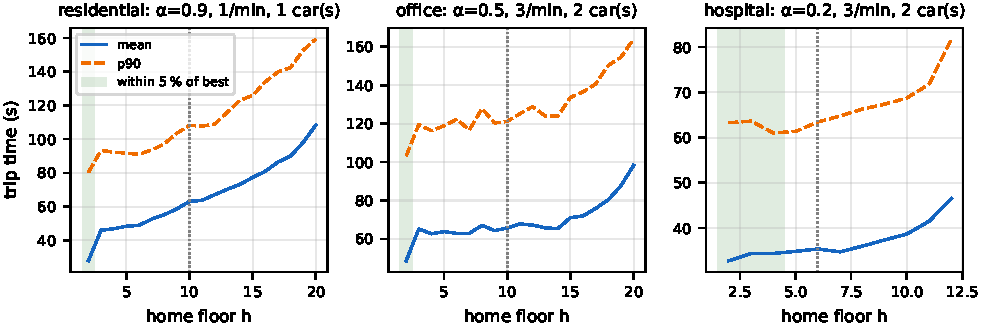
\includegraphics[width=\textwidth]{figures/regret.pdf}
\caption{Three archetypes with stairs on: mean and 90th-percentile trip time
by home floor, the 5\% indifference band (shaded) and the middle floor
(dotted).}
\label{fig:arch}
\end{figure*}

Three archetypes make it concrete (Figure~\ref{fig:arch}). A
\emph{residential} tower (\ArcResidentialN\ floors, $\alpha = 0.9$, one car,
1/min): optimum floor \ArcResidentialH, band \ArcResidentialBand, the middle
floor \ArcResidentialRegMid\% worse and the top floor
\ArcResidentialRegTop\% worse; the p90-optimal floor is the same. An
\emph{office} (\ArcOfficeN\ floors, $\alpha = 0.5$, two cars, 3/min): optimum
\ArcOfficeH, middle-floor regret \ArcOfficeRegMid\%, \ArcOfficeWalked\% of
trips walked. A \emph{hospital}-like building (\ArcHospitalN\ floors, $\alpha
= 0.2$, two cars, 3/min, cars parked mid-building): optimum \ArcHospitalH\
with a band of \ArcHospitalBand, middle-floor regret \ArcHospitalRegMid\%,
p90-optimal floor \ArcHospitalHp\ --- the one case where the floors are close
to interchangeable and the tail, not the mean, should pick.

The rule of thumb that survives all of this: count how often you leave the
building against how often you move within it. If leaving dominates, the
lowest floor you can get wins by a wide margin, the elevator's parking policy
is the next most important thing, and the stairs make the low floor better
still. If moving within dominates and the cars are busy, live anywhere from
the middle up and stop worrying.
